\documentclass[conference]{IEEEtran}
% *** MATH PACKAGES ***
%\usepackage[cmex10]{amsmath}
\usepackage{amsmath}
\usepackage{amssymb}
% correct bad hyphenation here
\hyphenation{op-tical net-works semi-conduc-tor}
% Utilisation des accents
\usepackage[utf8]{inputenc}
% liens hypertext
\usepackage{hyperref}
% Images
\usepackage{graphicx}
% Code Java
\usepackage{listings}
\usepackage{color}

\definecolor{dkgreen}{rgb}{0,0.6,0}
\definecolor{gray}{rgb}{0.5,0.5,0.5}
\definecolor{mauve}{rgb}{0.58,0,0.82}

\lstset{frame=tb,
  language=Java,
  captionpos=b,
  aboveskip=3mm,
  showstringspaces=false,
  columns=flexible,
  basicstyle={\small\ttfamily},
  numbers=none,
  numberstyle=\tiny\color{gray},
  keywordstyle=\color{blue},
  commentstyle=\color{dkgreen},
  stringstyle=\color{mauve},
  breaklines=true,
  breakatwhitespace=true,
  tabsize=3
}

\begin{document}

% paper title
% can use linebreaks \\ within to get better formatting as desired
% Do not put math or special symbols in the title.
\title{Paradigme de programmation par agents}

% author names and affiliations
% use a multiple column layout for up to three different
% affiliations
\author{
\IEEEauthorblockN{David Levayer}
\IEEEauthorblockA{Étudiant en maîtrise à l'Université\\du Québec à Chicoutimi,\\
Élève ingénieur à Polytech Grenoble\\
Contact : david.levayer [at] gmail.com}
\and
\IEEEauthorblockN{Corentin Ricou}
\IEEEauthorblockA{Étudiant en maîtrise à l'Université\\du Québec à Chicoutimi,\\
Élève ingénieur à Polytech Grenoble\\
Contact : corentin.ricou [at] gmail.com}
}

\maketitle

\begin{abstract}
\fontsize{10pt}{12pt}\selectfont
\textmd{
Le document suivant est réalisé dans le cadre du cours ``Patrons et modèles" de H. Mcheick à l'Université du Québec à Chicoutimi. La programmation par agents est un paradigme de programmation proposée il y a une quinzaine d'années. Elle vient palier les défauts de la programmation orientée-objet notamment pour le développement d'applications distribuées. Le développement d'agent est particulièrement pertinent si l'on souhaite disposer d'un réseau d'entités dynamiques et \textit{context-aware}. Certains environnements profitent largement des caractéristiques particulières de ce type de programmation. Cet article présente brièvement le concept d'agent et propose une approche expérimentale basée sur le framework Jade. Il revient également sur les forces et les faiblesses de ce modèle et sur son intérêt en tant que patron architectural.\\
}
\end{abstract}

\begin{IEEEkeywords}
\textmd{
Pattern, Object-oriented-programmation, Agent, Multi-agent system, Distributed application, Mobile, Adaptation, Jade}
\end{IEEEkeywords}

% For peer review papers, you can put extra information on the cover
% page as needed:
% \ifCLASSOPTIONpeerreview
% \begin{center} \bfseries EDICS Category: 3-BBND \end{center}
% \fi
%
% For peerreview papers, this IEEEtran command inserts a page break and
% creates the second title. It will be ignored for other modes.
\IEEEpeerreviewmaketitle

\section{Introduction}

Depuis maintenant une quinzaine d'années \cite{garneau}, la programmation orientée-agent se démarque et s'affirme comme une évolution pertinente à la programmation orientée-objet. De part l'essor des moyens de communication et grâce à des capacités réseaux toujours plus élevées, le développement d'applications distribuées prend tout son sens. Il permet une meilleure répartition des tâches entre les individus d'un même réseau et offre de généralement un meilleur temps d'exécution. Les systèmes sont ainsi répartis sur plusieurs machines et interagissent entre eux : ils sont à la fois autonome et conscient de leur environnement. Ce dernier évolue au cours du temps et il est important de tenir compte de ces variables au cours de l'exécution.\\

Ce caractère dynamique et évolutif est au coeur de la programmation orientée-agent. Dans l'optique de faciliter le développement et l'intégration de tels systèmes, plusieurs \textit{frameworks} ont été développés afin de supporter au mieux ce paradigme de programmation. Jade est l'un d'entre eux : ce framework développé en Java permet de faciliter et de standardiser le développement de système multi-agents. Dans un premier temps, cet article présente le contexte d'utilisation de la programmation orientée-agent avant de décrire plus en détails les caractéristiques de cette dernière. Nous présenterons ensuite le framework Jade avant de donner un prototype complet de système multi-agents. Une courte conclusion sera l'occasion de rappeler les différents avantages et les limites de cette approche.\\

\section{Contexte d'utilisation}

De nos jours, Internet est en constante évolution. Si le Web 2.0 favorise les interactions \textit{Human-to-Human}, le Web 3.0 pourrait très bien être celui des interactions \textit{Machine-to-Machine} \cite{boissier}. L'essor des systèmes distribués et des intelligences artificielles requiert une évolution dans la façon de penser et de concevoir des systèmes à la fois dynamiques, intelligents et déployables à grande échelle. De ces besoins est né le concept d'agent : la création d'une entité autonome destinée à accomplir une tâche précise en fonction d'un environnement donné.\\

Même si ce concept prend tout son sens dans les systèmes distribués, on peut noter qu'il se démarque également dans d'autres contextes spécifiques. C'est notamment le cas lorsque le nombre de données à partager est très important ou lorsque la bande passante du réseau est faible. Dans les deux cas, l'envoi d'un agent ``sur place" limite l'utilisation du réseau en privilégiant une résolution locale du problème. Les réseaux à grande latence (communication satellite par exemple) ou non-fiables (coupures fréquentes) sont également de bons exemples d'environnements où le déploiement d'agents possède un avantage certain. Enfin, on peut ajouter que l'utilisation d'agents peut être interessante lorsque les traitements réalisés ont une relation de causalité : l'agent évolue et se déplace dans un nouveau contexte en tenant compte des informations qu'il a accumulé lors de ces précédents traitements.\\

\section{Programmation par agents}
\vspace*{1mm}

\subsection{Présentation générale}
\vspace*{1mm}

En informatique, un agent est une entité logicielle qui agit de façon autonome. S'il est mobile, il peut également se transférer d'un environnement à un autre par ses propres moyens. Il interagit alors avec les services fournis par l'environnement et tente d'accomplir un but préalablement défini \cite{gray}. Malgré leur caractère autonome, les agents communiquent entre eux afin d'acquérir et de partager de l'information. Idéalement, un agent possède un seul but. Ce dernier peut néanmoins être divisé en une multitude de sous-objectifs. Fait important, un agent est par ailleurs soumis à un cycle de vie : il naît (instanciation), réalise sa tâche (vie de l'objet agent) et meurt (libération mémoire lorsque la tâche est accomplie). Cette vision d'un agent est très importante car elle est l'analogie d'un être humain. De la même façon que la modélisation objet est basé sur la représentation des objets réels qui nous entourent, le concept d'agent représente une personne réelle. Comme tout être humain, un agent est donc autonome, pensant et en constante interaction avec son environnement. Il prend des décisions afin d'accomplir au mieux la tâche qui lui est confiée.\\

\subsection{Différence entre agent et agent mobile}
\vspace*{1mm}

Tous les agents ne sont pas des agents mobiles. Un agent ``classique" s'exécute intégralement depuis l'environnement dans lequel il a été crée alors qu'un agent mobile peut être amener à se déplacer vers un autre environnement. Ainsi, un agent mobile ``s'envoie" vers l'environnement cible puis est reconstruit (nouvelle instance) afin de s'exécuter en local (traitement réalisé sur la machine hôte). Pour accomplir ses objectifs et récolter des informations, un agent classique va quant à lui communiquer de manière accrue, notamment avec d'autres agents distants. Ces échanges prennent le plus souvent la forme de messages. On perd alors certains avantages propres aux agents mobiles, notamment l'économie de bande passante ou le caractère ``hors-ligne" de certaines opérations. En revanche, on conserve les avantages propres à la programmation par agent (et à la programmation distribuée de manière plus large) : réduction du temps total d'exécution, réduction du temps de réponse (parallélisme), équilibrage des charges ou encore déploiement dynamique. Les figures Fig.~\ref{fig:classique} et Fig.~\ref{fig:mobile} illustrent les schémas d'exécution de ces deux types d'agents. Le framework Jade présenté ci-après propose un modèle d'agent non-mobile. Lorsqu'un agent veut des informations sur un contexte distant, il envoie un message via le système de messagerie intégré au framework.\\

\begin{figure}[h]
\centering
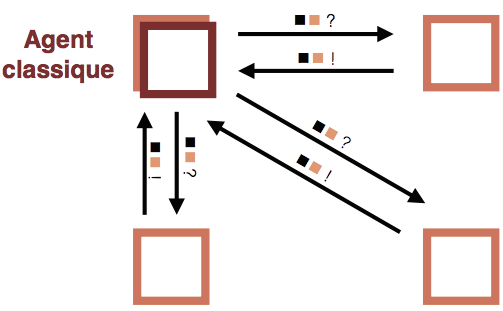
\includegraphics[width=170pt]{images/classique.png}
\caption{Schéma d'exécution d'un agent classique}
\label{fig:classique}
\end{figure}

\begin{figure}[h]
\centering
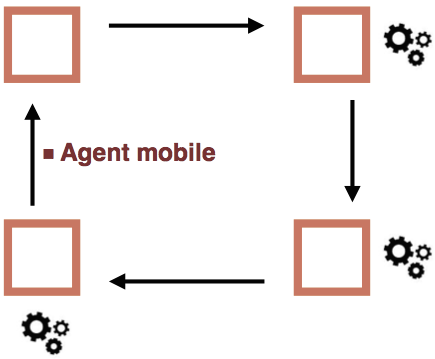
\includegraphics[width=170pt]{images/mobile.png}
\caption{Schéma d'exécution d'un agent mobile}
\label{fig:mobile}
\end{figure}

\subsection{Agents, patrons et modèles}
\vspace*{1mm}

Plusieurs patrons de programmation et de conception peuvent être identifiés lorsque l'on souhaite programmer des agents de manière simple et efficace. On peut notamment noter les patrons Observer, Strategy ou encore Visitor. Ces patrons simplifient grandement la programmation par agent en fixant un cadre propre et concret. On peut supposer que les frameworks tels que Jade intègrent ces patrons. Il convient également de noter qu'il est possible (et conseillé) d'implémenter un patron à l'intérieur d'un agent. Prenons l'exemple du patron Observer : il suffit d'ajouter une méthode \textit{notify} à l'agent ``modèle". Cette méthode contacte les agents observateurs via le système de messagerie. Chaque observateur doit de son côté définir une méthode \textit{update} qui met à jour l'agent en fonction du nouveau modèle.\\

Il est important de noter que Jade fournit un système de \textit{behavior} pour programmer des agents. Cet outil facilite la séparation des préoccupations et permet également d'ajouter (et de réutiliser) facilement un patron de programmation (en l'ajoutant à un agent sous forme d'un nouveau comportement). Le fonctionnement des \textit{behavior} est décrit plus en détails dans la suite de ce document. Pour terminer, on peut affirmer que le paradigme de programmation par agents est lui-même un patron architectural. En effet, il apporte une solution à des problèmes récurrents : programmer efficacement des applications distribuées, rendre un système dynamique et autonome ou encore palier les limites de l'environnement (réseau non-fiable, faible bande passante, grande latence, etc).\\

\section{Framework Jade}

Jade (Java Agent Development Framework) est un framework logiciel développé dans le langage Java \cite{jade}. l'objectif affiché est simple : fournir un ensemble d'outils destinés à faciliter la programmation par agents. Jade fournit pour cela un \textit{middleware} permettant de déployer des agents via une interface graphique. Les agents peuvent être répartis sur plusieurs machines hétérogènes (systèmes d'exploitation différents) ; ils sont alors contrôlés à distance. Les avantages de Jade sont multiples : il est \textit{open-source}, facile à prendre en main et facile à utiliser. Il dispose par ailleurs d'une grande communauté et de nombreuses APIs. Il convient de noter que Jade requiert au minimum la version 5 de l'environnement Java (JDK) pour fonctionner.\\

L'outil Jade fournit également un système de messagerie avancé. Ce dernier permet aux agents de communiquer entre eux via des messages. Chaque message contient des données (contenu du message) et des méta-données (destinataire, expéditeur, type de message, etc). Ce module respecte les normes FIPA (Foundation for Intelligent Physical Agents). Cette organisation, membre de l'IEEE, a pour but de définir promouvoir l'utilisation de systèmes multi-agents et de garantir l'inter-opérabilité de ces derniers, notamment en fixant des standard de communication. Les avantages de cette norme permettent notamment aux agents ``Jade" de communiquer avec des agents d'un autre framework (dès lors que ce dernier respecte lui aussi les normes FIPA).\\

\begin{figure}[h]
\centering
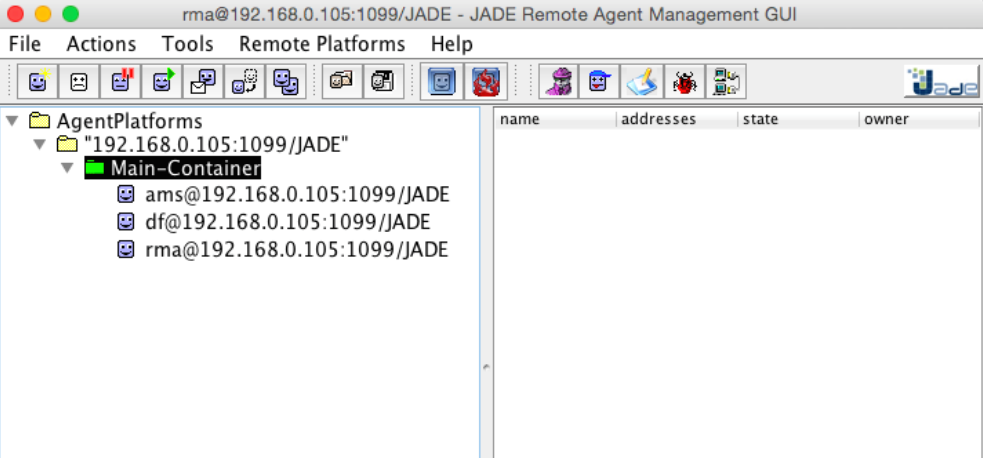
\includegraphics[width=240pt]{images/jade.png}
\caption{Capture d'écran de l'interface fournie par Jade}
\label{fig:jade}
\end{figure}

les agents lancés par Jade sont placés à l'intérieur de containers (figure Fig.~\ref{fig:jade}) Chaque container correspond à un environnement particulier. Les communications à l'intérieur d'un même container sont simplifiés ; néanmoins, il est tout à fait possible de communiquer avec des agents présents dans un autre container. Cette modélisation permet d'accentuer la séparation des préoccupations : on peut ainsi créer un container par application et lancer plusieurs applications dans la même interface. Il est également possible (toujours via l'interface) d'ajouter un \textit{remote container}. Deux conséquences majeurs résulte de l'ajout d'un container distant : il est possible de configurer (et de lancer) des agents à distance (sur le-dit container) et il est possible d'interagir avec les agents distants présents (envoi de messages). Cette partie du framework garantit donc la possibilité de développer facilement des applications distribuées.\\

\begin{lstlisting}[caption=Création d'un agent, label=lst:agent, float=t]

import jade.core.Agent;

public class MyAgent extends Agent {

    // Agent fields
    private int myAttribut;
    
    // Called when an agent is created
    protected void setup() {
    
        // Agent initialisation
    }    
}
\end{lstlisting}

Jade met à disposition de puissants outils permettant de construire des agents de manière modulaire. La création d'un objet de type agent est très simple et passe par un simple héritage (code List.~\ref{lst:agent}). L'initialisation d'un agent comprend souvent l'ajout de comportements, ou \textit{behaviors}. Un comportement définit les actions réalisables par l'agent et les conditions de réalisation. Un comportement doit définir deux méthodes ; la première est appelée lorsque l'on souhaite exécuter le code correspondant au comportement (action). La seconde permet de savoir si le comportement (et les actions associées) est achevé. La programmation de comportements est très modulaire et permet une large réutilisation de code. On peut partager certains comportements entre différents agents, notamment si l'on souhaite intégrer des patrons de programmation. On pourrait par exemple imaginer un comportement \textit{Observer} qui contiendrait le code du patron du même nom. Le code List.~\ref{lst:behavior} illustre la structure d'un comportement avec Jade.\\

\begin{lstlisting}[caption=Agents et comportements, label=lst:behavior]

import jade.core.Agent;
import jade.core.Behavior;

// Put this code into the Agent class
// for example in setup() method
addBehavior(new MyBehavior());

// Class which define the behavior
private class MyBehavior extends Behavior {

    // Behavior fields
    private int myAttribut;
    
    @Override
    public void action() {
    
            // Behavior code
    }
    
    @Override
    public boolean done() {
    
            // true if the behavior is done
            // false otherwise
    }
}
\end{lstlisting}

\section{Prototype réalisé}

Le contexte choisi pour la réalisation d'un système multi-agents est décomposé en deux parties. La première est composée d'agents appelés ``stations". Une station comprend différents capteurs et offre plusieurs services. Le choix des capteurs est propre à chaque station, de même que le choix des services à implémenter\footnote{Dans notre implémentation de ce problème, toutes les stations fournissent les mêmes services.}. Une station ne meurt (désallocation de l'agent) que si l'utilisateur le demande ; autrement, elle se contente d'attendre des demandes d'agents et de les traiter. La seconde partie est constituée d'agents ``explorateurs". Un explorateur est créé avec plusieurs paramètres : le service qu'il recherche et, si besoin est, les capteurs associés. Le comportement de cet agent est plutôt simple : il commence par rechercher les stations présentes dans son environnement. Pour chaque station, il envoie un message indiquant qu'il souhaite accéder à l'un des services de la station. Si ce service requiert une liste de capteurs, il fournit la liste spécifiée lors de sa création. Les fonctionnalités offertes utilisent le concept de \textit{behavior} fourni par Jade (valable pour les deux catégories d'agents).\\

Les services proposés par les stations sont relativement simples mais ils sont suffisant pour démontrer le potentiel du framework Jade. On trouve ainsi quatre services : demander le nom de la station, demander les capteurs disponibles sur la station, demander les dernières valeurs des capteurs de la station et demander toutes les valeurs des capteurs de la station. Les deux derniers services requièrent que l'explorateur spécifie les capteurs qui l'intéresse. L'ensemble des communications est réalisé grâce à des messages ACL (\textit{Agent Communication Language}). La nature et les paramètres de chaque requête sont codifiés dans le contenu du message (code pour le type de service et codes pour identifier les capteurs d'intérêt).\\

Enfin, nous avons choisi de programmer deux interfaces graphiques afin de simplifier la configuration des agents. Ces interfaces permettent de spécifier les paramètres de lancement des agents mais également de la modifier durant l'exécution. On peut ainsi spécifier les capteurs disponibles sur une station ou préciser la tâche que doit accomplir un explorateur. Les figures Fig.~\ref{fig:station} et Fig.~\ref{fig:explorer} montrent les deux interfaces disponibles. Pour exécuter le prototype, il suffit de réaliser les étapes suivantes :\\

\begin{enumerate}

  \item Récupérer les fichiers sources du prototype ainsi que les librairie de Jade (\textit{jade.jar} et \textit{commons-codec-1.3.jar}). L'ensemble de ces fichiers est disponible à l'adresse suivante : \href{https://github.com/DavidLevayer/JadeProject}{[Projet Jade]}. Les étapes 2 et 3 supposent que les librairies sont placées dans le sous-dossier ./lib.\\
  
  \item Compiler les classes contenant les agents à utiliser (si ce n'est pas déjà le cas). On suppose que les agents en question sont dans /src/collector. Il suffit d'ouvrir un terminal et de saisir la commande suivante :
  \begin{lstlisting}[language=bash,frame=none]
  $ javac -cp lib/jade.jar -d classes src/collector/*.java
  \end{lstlisting}

  \item L'étape suivante consiste à démarrer l'interface principale de Jade (Fig.~\ref{fig:jade}). On part du principe que les classes compilées à l'étape précédente sont présentes dans le dossier ./classes. La commande suivante est alors utilisée pour lancer Jade :
  \begin{lstlisting}[language=bash,frame=none]
  $ java -cp lib/jade.jar:classes/ jade.Boot -gui
  \end{lstlisting}
  
  \item Pour lancer les agents, il ne reste plus qu'à se placer dans le container choisi et créer un nouvel agent (en cliquant sur l'icône correspondante ou dans le menu contextuel accessible après un clic droit sur le container).
  
\end{enumerate}

\begin{figure}[h]
\centering
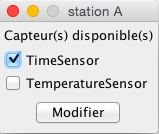
\includegraphics[width=120pt]{images/station.png}
\caption{Interface graphique d'une station}
\label{fig:station}
\end{figure}

\begin{figure}[h]
\centering
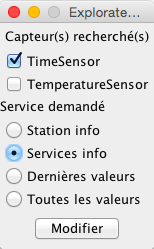
\includegraphics[width=120pt]{images/explorer.png}
\caption{Interface graphique d'un explorateur}
\label{fig:explorer}
\end{figure}

\section{Conclusion}

La programmation par agent est un véritable paradigme de programmation. Elle permet de modéliser un problème via un ensemble dynamique d'entités autonomes appelées agents. On peut faire une analogie entre un agent et un être vivant : il naît, accomplit son but puis meurt. Le framework Jade offre un panel d'outils permettant de développer des agents de manière simplifiée et en respectant les standards de l'IEEE. L'interface graphique du framework permet de répartir aisément les agents sur différentes plateformes hétérogènes, ce qui est largement appréciable pour le développement d'applications distribuées.\\

La programmation par agent peut être vue comme un véritable patron architectural. Elle permet de résoudre plusieurs problèmes clés (souvent liés au réseau) tels que la préservation de la bande passante, la réduction des latences réseaux, la réduction du temps d'exécution ou encore la réparation des charges à l'intérieur d'un système complexe. Le développement d'agents est par ailleurs largement basé sur plusieurs patrons de programmation (encapsulés dans le code du framework) et n'empêche en rien la programmation de patrons de conception ``par dessus" la couche agent. C'est donc un outil de choix pour le développement d'applications distribuées.\\

\begin{thebibliography}{56}

\bibitem{garneau}
T. Garneau and S. Deliste, \emph{Programmation orientée-agent : évaluation comparative d'outils et environnements}, JFIADSMA, Lille, France, 28-30 octobre 2002.

\bibitem{boissier}
O. Boissier, \emph{Multi-agent system}, support de cours, http://www.emse.fr/~boissier/enseignement/maop11/courses/introduction-4pp.pdf, consulté le 21 avr. 2015.

\bibitem{gray}
R. Gray, D. Kotz, G. Cybenko and D. Rus, \emph{Mobile agents: Motivations and state-of-the-art systems}, Tahyer School of Engineering, Dartmouth College, 2000.

\bibitem{jade}
TILAB, \emph{Jade Website}, http://jade.tilab.com, consulté le 2 avr. 2015.

\end{thebibliography}

% that's all folks
\end{document}


